\section{Qualitätsszenario}

\begin{tcolorbox}[title=Qualitätsszenario]

    Bleiben Qualitätsindikatoren zu abstrakt, ist für die Qualitätssicherung häufig unklar, was genau zu überprüfen ist.\\
    Aus diesem Grund werden Qualitätsforderungen mittels \textbf{Szenarien} exakter beschrieben und für die Praxis damit nutzbar.\\
    Ein \textbf{Qualitäts-Szenario} besteht aus folgenden Teilen (s. Abbildung:~\ref{fig:qualitätsszenario}):

    \begin{enumerate}
        \item \textbf{Quelle des Stimulus}: \textit{Akteur} (Mensch, Computersystem, Hardware)
        \item \textbf{Stimulus}: \textit{Vorgang}, der etwas im System auslöst
        \item \textbf{Umgebung}: Der \textbf{Stimulus} tritt in einer Umgebung auf (bspw. ``System, mit dem 100 Benutzer gleichzeitig arbeiten``)
        \item \textbf{Artefakt}: Das gesamte System oder Teile davon (die \textit{Dokumentation} gehört auch dazu)
        \item \textbf{Antwort}: Die \textit{Aktivität}, die auf den \textbf{Stimulus} hin erwartet wird
        \item \textbf{Messvorschrift}: eine genau definierte \textit{Messung}, also so, dass sie \textit{objektiv messbar} ist
    \end{enumerate}

\end{tcolorbox}

\begin{figure}
    \centering
    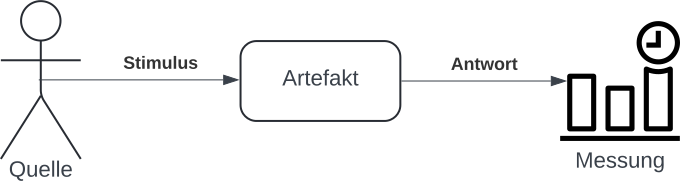
\includegraphics[scale=0.4]{part four/Qualität/img/qualitätsszenario}
    \caption{Skizze eine \textit{Qualitätsszenarios}. Eine \textbf{Umgebung}, in der der Stimulus auftritt, wird implizit vorausgesetzt. (Quelle: in Anlehnung an~\cite[Abb. 1.2, 4]{Wed09c})}
    \label{fig:qualitätsszenario-cc}
\end{figure}
